\chapter{Introduction}

This chapter introduces the research topic, provides an overview and motivation for the study, and outlines the main objectives and expected outcomes. It also outlines the methodology and briefly describes how the rest of the report is organized.

\section{Project Overview}
Ordinary Differential Equations (ODEs) describe how a system change with over time. They are widely used in fields such as physics, engineering, and mathematics. In many 
real-world problems, particularly those involving complex or nonlinear equations, it is often 
not possible to obtain exact solutions. That is why methods such as Euler’s method and 
Runge-Kutta are used to obtain approximate solutions. In this project, we examine a 
particular system consisting of three nonlinear equations known as the Lorenz-1960 system 
(one of the first meteorological models). The system is small, but complex enough to 
make a good testing ground for various solution methods. The Lorenz-1960 system is a 
great candidate for evaluating how well  artificial neural network (ANN) learn and predict behavior. Classical 
numerical methods address these problems step by step. Also they are typically accurate, but 
they are very slow and require more computational cost. We use numerical methods like Runge-Kutta to generate data that can be used to train artificial neural networks to learn how variables change over time.
The ANN learns to match its predictions with the results of the numerical solver during training. After training, the ANN can quickly predict results for any time without solving the equations again.
Therefore, the primary aim  of this project is to solve the Lorenz-1960 system 
and to see how well a plain ANN can learn its behavior and which ANN architecture provides
optimal results. 


\section{Motivation}
This project is research and application driven. Classic numerical methods have been tested and proven to be accurate and reliable. They work well for directly simulating equations. A trained artificial neural network (ANN), on the other hand, can solve the equation on its own. It forecasts and behaves as a copy of the actual system. Numerous investigations are currently used: Solving differential equations with neural network approximators based on PINNs, operator learning and ANN. This makes the topic interesting and relevant to investigate. Another motivation for this project is the learning and hands-on benefits it offers. It offers the building of skills in solving an ordinary differential equation(ODEs). It also provides training on how to construct and utilize models of the neural network. The project involves running experiments and analysing results. It's useful to compare different methods. Although simple ANNs are not as powerful as advanced methods, they will give us some insights into their abilities and limitations.



\section{Objectives}
The main aims of this project are:


\begin{itemize}
    \item  To numerically solve a coupled and nonlinear system (Lorenz equation).

\end{itemize}

\begin{itemize}
    \item To apply ODE concepts, numerical methods such as the Runge-Kutta and SciPy solvers, The Lorenz equations are solved using an ANN. Numerical solutions obtained from the Runge-Kutta method.


\end{itemize}

\begin{itemize}
    \item To generate accurate data with the Runge-Kutta method and then verify the numerical solutions with it. Compare and evaluate the performance of ANN.
    
\end{itemize}

\begin{itemize}
    \item To compare the different ANN architecture to varying the number of layers, varying number of neurons per layer and testing various activation functions to determine the most optimum one.

\end{itemize}

\begin{itemize}
    \item To evaluate the model’s performance we are using mean squared error, learning stability, and other measures, we assessed the performance of the model. See if a plain ANN can learn the Lorenz equation and explore the trade off between the two variables, namely computational cost.

\end{itemize}

\begin{itemize}
    \item To compare the results with PINN based methods from other research to understand how this approach performs compared to recent techniques.
\end{itemize}


\section{Methodology}
The “Waterfall Methodology” is being followed. Here, the various phases are carried out one after the other in a fixed order. It is fitting as we know what we want and need from the outset. In this, the input of each step is the output of the next step. This helps the process to be structured, easy to track and easy to manage.
       
       
       
       In the Literature Review phase the Lorenz-1960 equation and its property was studied.
Brief review of numerical methods, such as RK4, SciPy solvers. Besides, a number of ANN architectures, activation functions and training techniques were also investigated.
     
      
      
      The problem of the study and the objectives of the study were well stated in the Concept Development phase. The configuration of the layers in the ANNs was focused on approximation of the Lorenz-1960 equation, and the number of neurons, activation functions, learning rates and epochs of training were selected. Data sets for training and validation were prepared. 
      
      
      During the Design phase, ANN models and training strategy were developed, such as data processing and optimization of the network structure. The RK4 and SciPy were used to calculate a numerical baseline to compare with. Assessment measures, visualization tools, and statistical tests were set up to guarantee a valid comparison of models. Some statistical tests were also outlined to ensure appropriate comparisons between models. 
      
      
      During the Implementation phase numerical solvers and ANN models were developed. All of the models were trained using the datasets generated. The accuracy, training time, parameters number and convergence was measured. Each model was performed systematically based on the design. 
      
      In the Testing phase, we then tested the performance of each ANN model and then predicted
The results obtained by using the mean square error to evaluate its performance. We tested for generalization with new data. Compared the sensitivity of the models to various parameter values. The best models were compared with results from published studies. 


  Lastly, we have the Deployment phase, during which we incorporated all the results, plots, and analyses in the final project report. We designed and documented the code so that it was easy to repeat our work. The instructions for repeat experiments and retraining the models were included. We also presented our final suggestions on the best ANN architecture. This phase ensures that the project is complete and ready.
  




For better understanding, a diagram of our methodology is given below:-


\begin{figure}[h]
    \centering
    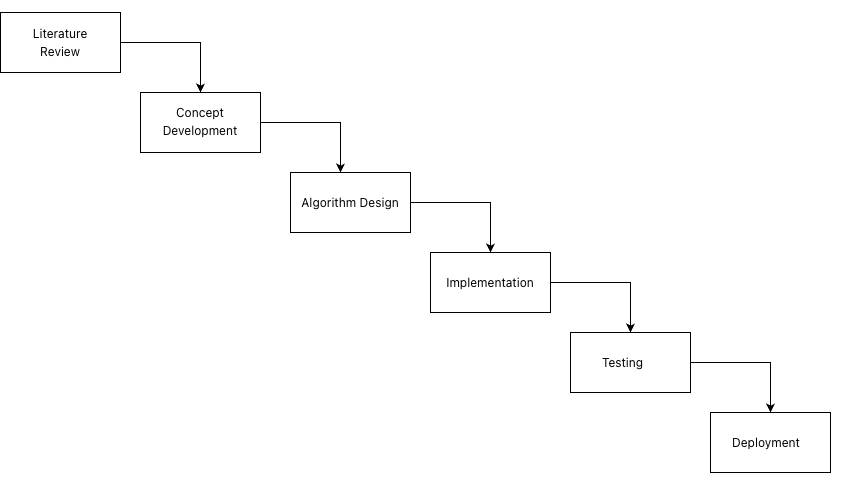
\includegraphics[width=0.8\textwidth]{Methodology.png}
    \caption{Methodology Diagram}
    \label{fig:methodology}
\end{figure}


\section{Project Outcome}
The expected outcome of the project will be the clear and the justified 
determination of the most appropriate architecture for the ANN in estimating 
the solution to the Lorenz-1960 system of ODEs within the scope of the experiment. This project must also include a 
numerical reference solution to the ODEs, the establishment of ANN 
baselines, and a comparative analysis of the results. \\[1pt]

The project will also contribute to the current understanding of the capacity
and limitations of ANN models in the approximation and solution of differential 
equations. If the ANN models are able to get a satisfactory level of accuracy in 
approximating the solution to the ODEs, the project will have demonstrated 
the capability of a simple ANN architecture to effectively act as an alternative 
numerical solver. This would suggest that a plain ANN, without the need for 
physics-informed loss terms or traditional mesh-dependent numerical 
methods, can on its own approximate ODE solutions with sufficient accuracy 
while being computationally less expensive in terms of inference time and the 
avoidance of iterative re-solving for each query. If the models do not achieve satisfactory accuracy in approximating solutions to the ordinary differential equations (ODEs), the study will clearly delineate the limitations of simple ANN architectures and mention the necessity for more advanced methods. \\[1pt]

This project will not only focus on coding and experiments, but also on understanding how different ANN structures, such as depth, width, and activation functions, influence the accuracy of solving coupled nonlinear ODE systems.



\section{Organization of the Report}
The rest of this report is outlined as follows. Chapter 2 outlines the theoretical 
background and literature review on Ordinary Differential Equations (ODE) 
solving, artificial neural networks, and existing neural methods for differential 
equations. Chapter 3 discusses about the project design, requirements, 
methodological plan, and task assignment. Chapter 4 outlines the 
implementation \& experiment design used in this research. Chapter 5 outlines 
the results and analysis on the tested ANN structures. Finally, Chapter 6 
concludes this report by focusing the main results, limitations, and potential 
directions for the future research. 
